
\documentclass[11pt]{beamer}
\usetheme{CambridgeUS}

\usepackage[utf8]{inputenc}
\usepackage[english]{babel}
\usepackage{amsmath}
\usepackage{amsfonts}
\usepackage{amssymb}
\usepackage{graphicx}
\usepackage{subfigure}
\usepackage{algorithm2e}
\usepackage{algorithmic}
\usepackage{url}
\usepackage{float}



% Puts the right page numbers for the presentation
\setbeamertemplate{footline}[frame number]

% Show uncovered items: 0 is invisible, 100 is fully visible
\setbeamercovered{transparent=3}

\author{Cody Eilar, Venkatesh Jatla, Mustafa Al-Mashhadani}
\title{Recommender Systems}
\logo{
\includegraphics[width=2.5cm]{figures/ecelogo.jpg}}
\institute{Dept of Electrical and Computer Engineering \\ The University of New Mexico \\ Albuquerque, NM 87131-0001, USA}
\date{\today}

\begin{document}
\maketitle
\section{Outline}
\begin{frame}
  \frametitle{Outline}
  \begin{itemize}
    \item Collaborative filtering
      \begin{itemize}
        \item Overview
        \item Data normalization
        \item Validation
        \item Results
        \item References
      \end{itemize}
    \item Content based filtering
      \begin{itemize}
        \item Block diagram
      \end{itemize}
  \end{itemize}
\end{frame}
\section{Collaborative filtering}


\begin{frame}
  \frametitle{Overview}
  \begin{figure}
    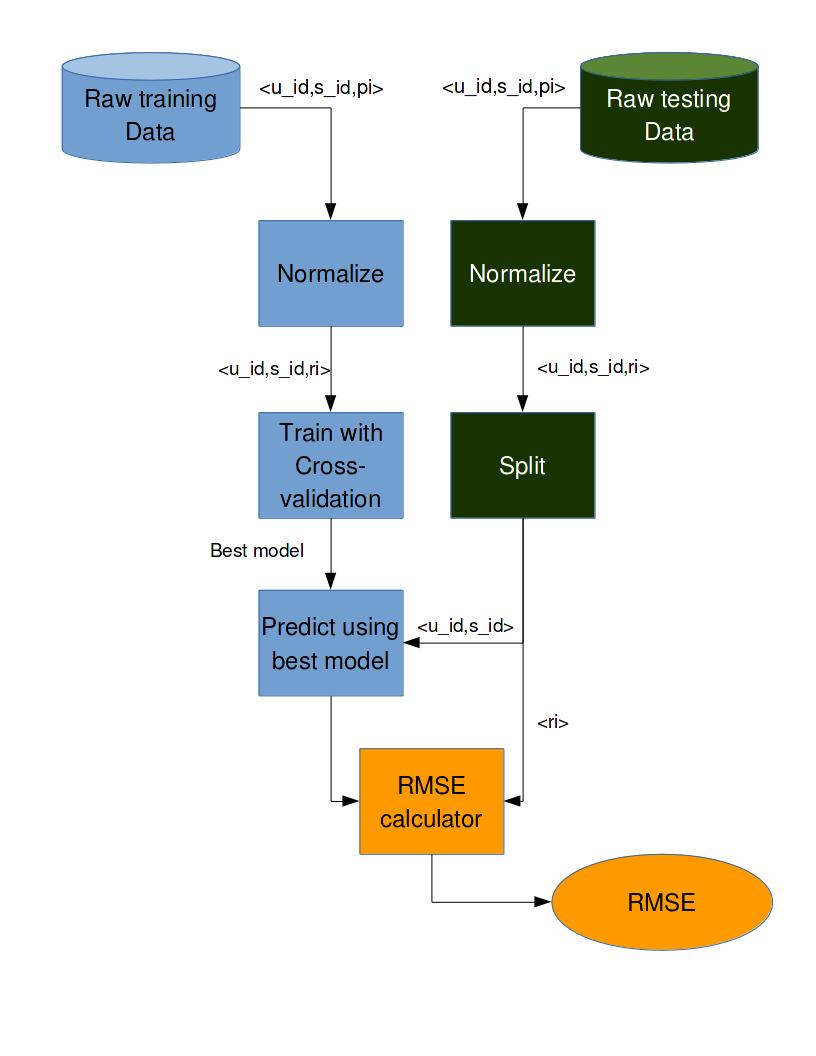
\includegraphics[width=0.5\linewidth]{figures/CollaborativeFilteringOverview.jpg}
  \end{figure}
\end{frame}


\begin{frame}
  \frametitle{Data normalization}
  \begin{itemize}
    \item Input Data = \{user\_id, song\_id, plays\}
    \item Normalize {\bf plays} so that
      \begin{itemize}
        \item 10 $=>$ Most liked song
        \item 0 $=>$ Most disliked song
      \end{itemize}
    \item If user $u_x$ has $P = \{p_1. p_2, p_3,\dots,p_n	\}$, then
      \begin{equation}
        r_i = 10 \times p_i/max\{P\}
      \end{equation}
  \end{itemize}
\end{frame}


\begin{frame}
  \frametitle{Validation block diagram}
  \begin{figure}
    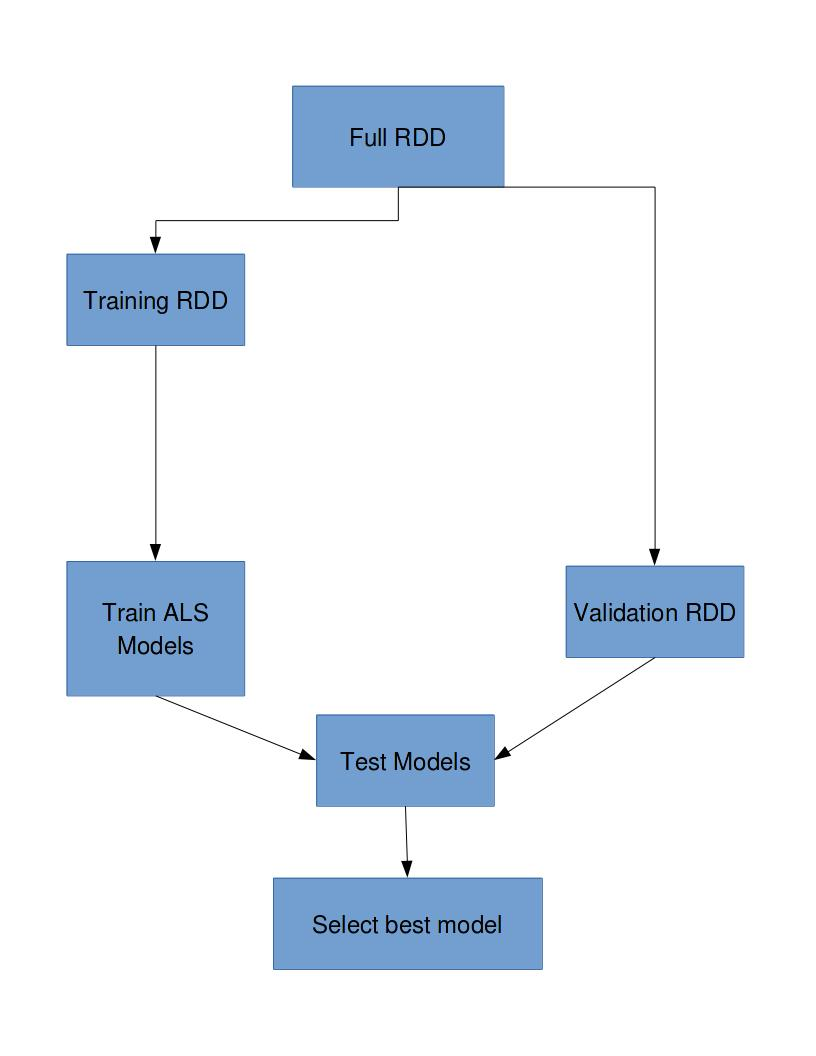
\includegraphics[width=0.5\linewidth]{figures/Validation.jpg}
  \end{figure}
\end{frame}


\begin{frame}
  \frametitle{Validation}
  \begin{itemize}
    \item Free parameters in ALS, \href{'http://spark.apache.org/docs/latest/mllib-collaborative-filtering.html'}{tutorial}
      \begin{itemize}
        \item rank, $\{R_0,R_1,\dots\}$
        \item lambda, $\{L_0,L_1,\dots\}$
        \item numIters, $\{N_0,N1,\dots\}$
      \end{itemize}
    \item Let input data RDD be, $R = \{row_i\}$, $row_i = \{user\_id_i, song\_id_i, r_i\}$
    \item Validation RDD is created by {\bf randomly sampling 10\%} of data RDD, $VS = 0.1R$
      \item Training RDD is creted by {\bf intersection compliment} of data RDD and Validation RDD,
        $TS = R - (R \cap VS)$
      \item Every possible combination is iterated and the model that gives {\bf minimum RMSE} on
        validation set, $VS$ is picked as best model.
    \end{itemize}
  \end{frame}
  \begin{frame}
    \frametitle{Results}
  \end{frame}


  \section{Content Based Filtering}
  \begin{frame}
    \frametitle{Getting Features}
    \begin{figure}[h]
      \centering
      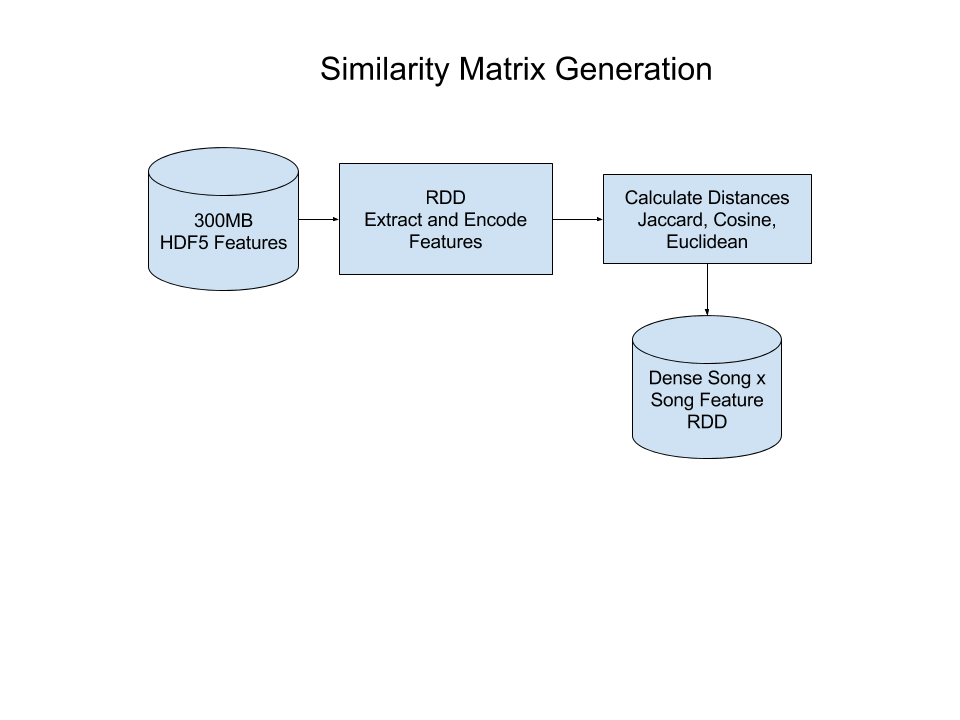
\includegraphics[width=4in]{figures/similarity_matrix.png}
      \caption{Extracting the features}
      \label{fig:similarity_matrix}
    \end{figure}
  \end{frame}

  \begin{frame}
    \frametitle{Generating Dense Rating Matrix}
    \begin{figure}[h]
      \centering
      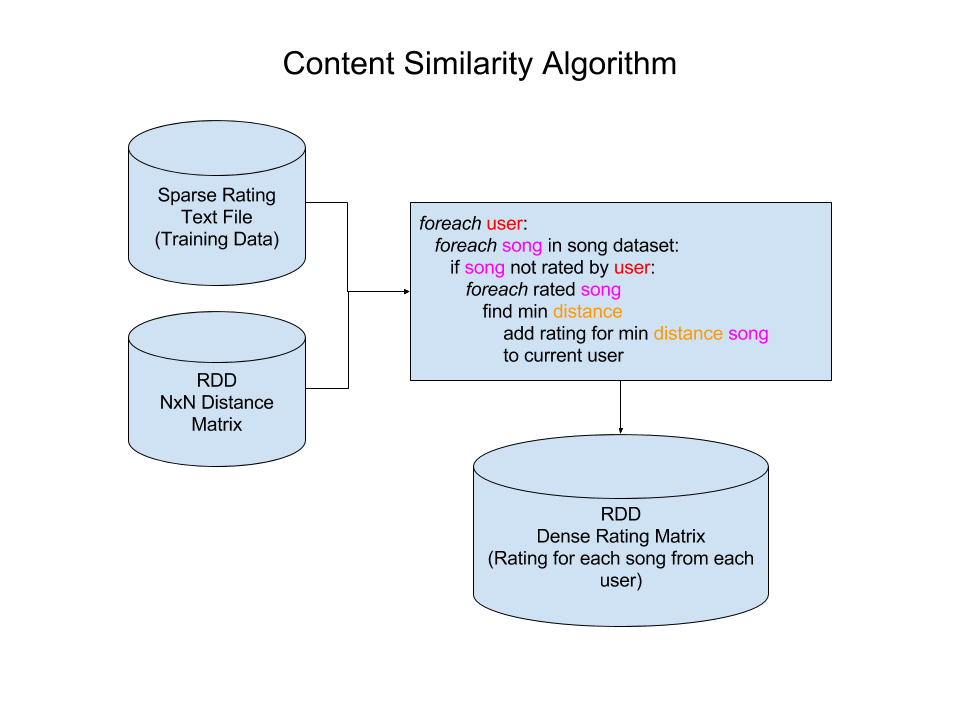
\includegraphics[width=4in]{figures/content_similarity_algorithm.png}
      \caption{Building a dense matrix to feed to the collaborative filtering algorithm}
      \label{fig:content_similarity_algorithm}
    \end{figure}
  \end{frame}

  \begin{frame}
    \frametitle{Combining Collaborative Filtering with Content Based Filtering}
    \begin{figure}[h]
      \centering
      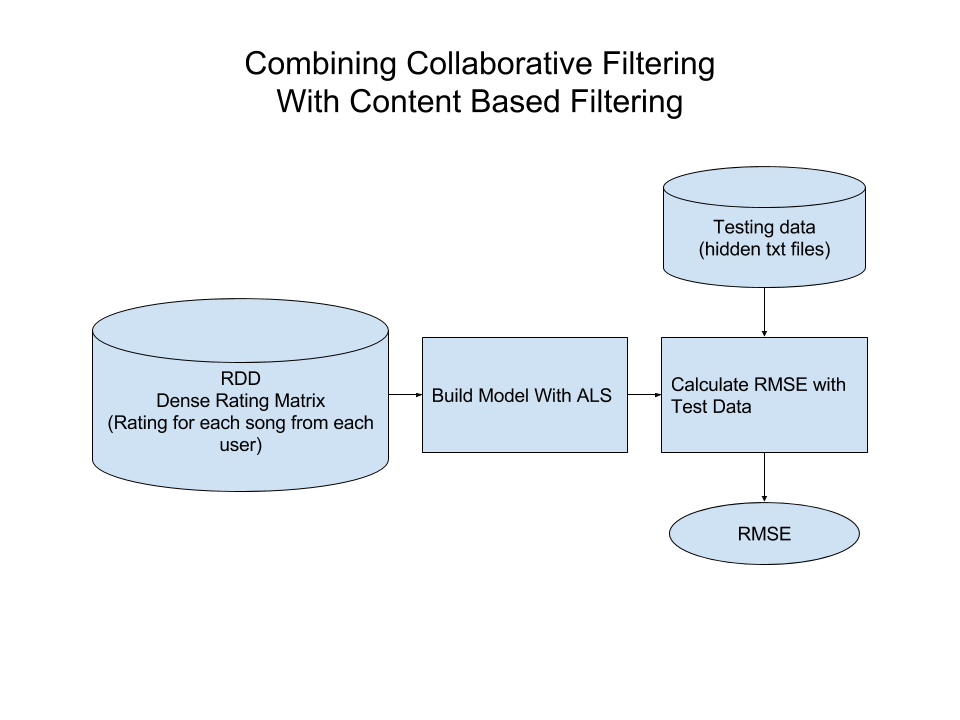
\includegraphics[width=4in]{figures/collab_plus_content.png}
      \label{fig:collab_plus_content.png}
    \end{figure}
  \end{frame}

  \end{document}
